	\begin{figure}[H]
		\centering
 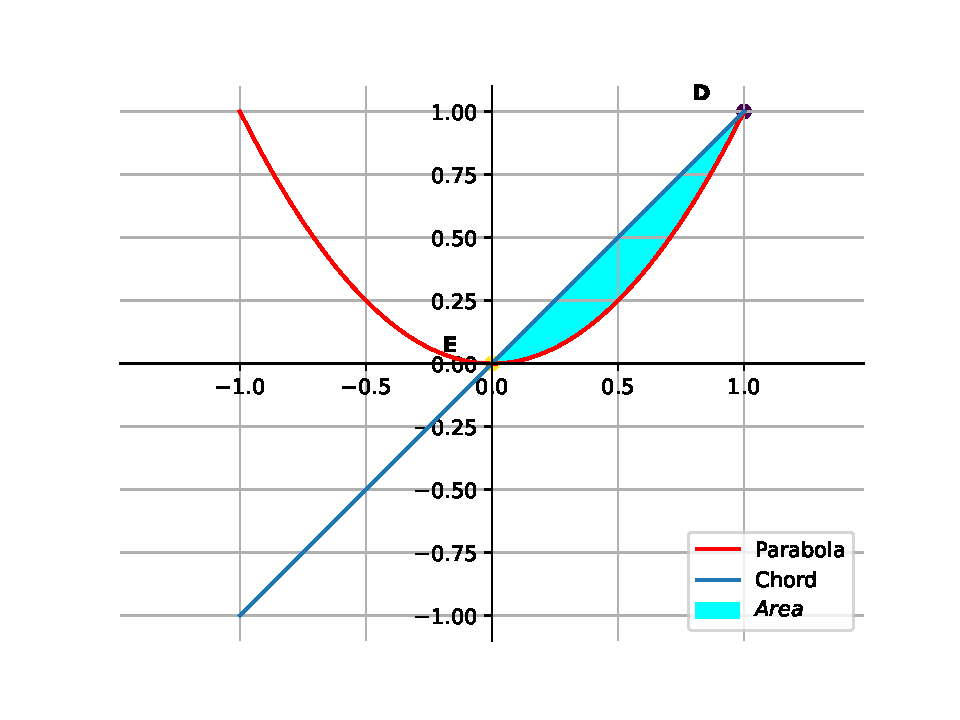
\includegraphics[width=0.75\columnwidth]{chapters/12/8/3/2/figs/fig.pdf}
		\caption{}
		\label{fig:12/8/3/2}
  	\end{figure}
The given curve  can be expressed as a conic with parameters
\begin{align}
	\vec{V} &= \myvec{1 & 0\\0 & 0}, \vec{u} = \myvec{0 \\-\frac{1}{2}}, f = 0
	\end{align}
The given line parameters are
\begin{align}
\vec{h} = \myvec{0 \\0}, \vec{m}=\myvec{1\\1}
\end{align}
Substituting the given parameters in 
\eqref{eq:tangent_roots},
\begin{align}
\vec{x}_1=\myvec{0\\0}, \vec{x}_2=\myvec{1\\1}.
\end{align}
From  
		\figref{fig:12/8/3/2},
the area bounded by the curve $y=x^2$ and line $y=x$ is given by
\begin{align}
	\int_{0}^{1} \brak{x 
	-\frac{x^2}{2}} \,dx = \frac{1}{6}
\end{align}
